%%=================================================================================
\begin{frame}{Systematics in statistical framework}
  Changing an energy correction factor (by systematic fluctuation) affects several parameters.
  For current results, it is assumed that {\bf only the parameter $X$ targetted by the systematic (POI) is affected} (hence fixing the others).

  Only the parametrization of $X$ will contain the measured uncertainty $\delta_X$ :
  $$X\rightarrow X(1+\delta_X\theta)$$
  with $\theta$ a gaussian constrained free parameter.
  \vfill
  \textcolor{red}{In the framework, the pulling of the nuisance parameters only affects the main parameter of the systematic}
\end{frame}

%%=================================================================================
\begin{frame}{Typical plot}
  \begin{minipage}{0.49\linewidth}
    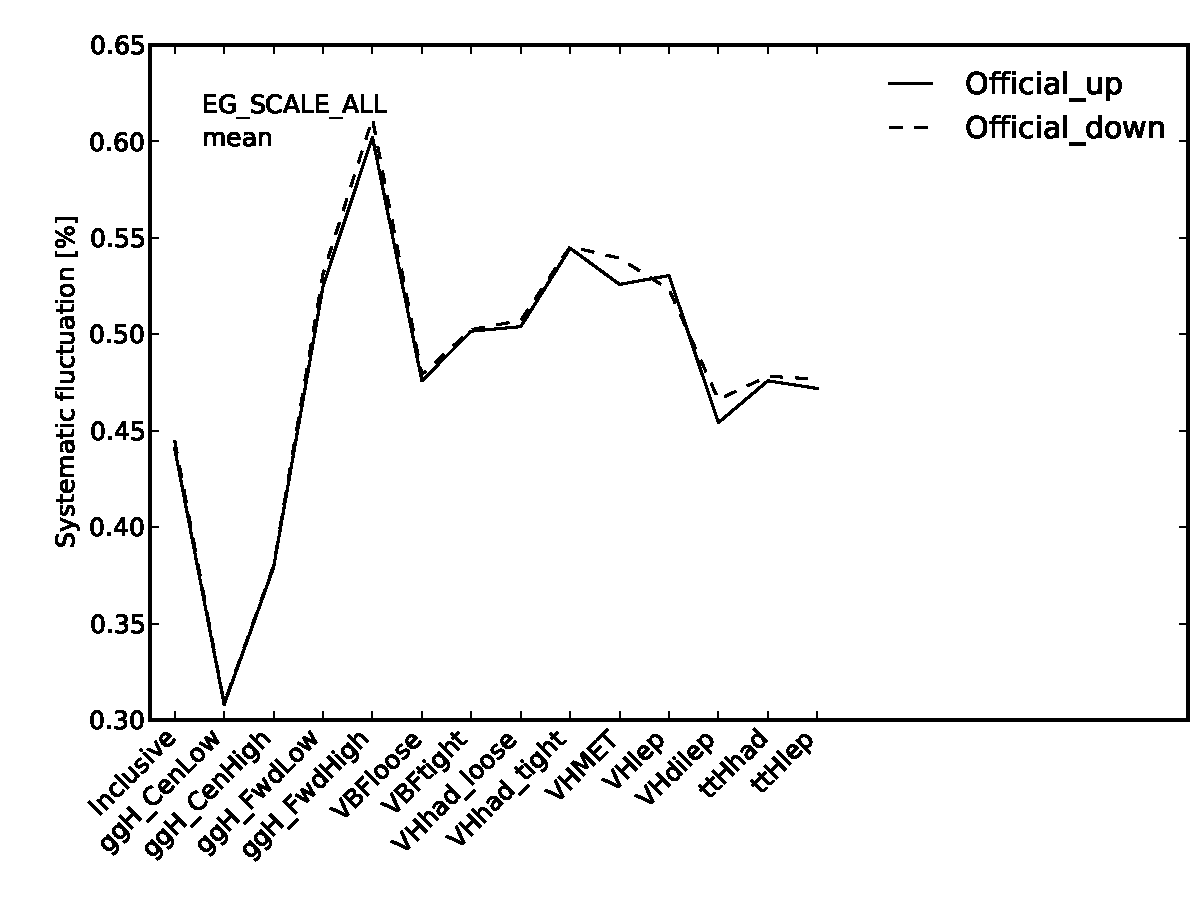
\includegraphics[width=\linewidth]{plots/Backup/h013_ICHEP_PhotonSyst_EG_SCALE_ALL_mean.pdf}\\
  \end{minipage}
  \begin{minipage}{0.49\linewidth}
    For a given fitted variable (here mean) :
    \begin{itemize}
    \item Full line : $\frac{\mu_{up}-\mu_{nominal}}{\mu_{nominal}}$
    \item Dashed line : $-\frac{\mu_{down}-\mu_{nominal}}{\mu_{nominal}}$
 
    \end{itemize}
  \end{minipage}

  Both lines should be superimposed in case of symmetric systematics.
  \end{frame}
%%=================================================%%=================================================================================
\begin{frame}{Scale impact on width}
  \begin{minipage}{0.49\linewidth}\includegraphics[width=\linewidth]{/home/goudet/Documents/LAL/Zim/Hgam/PhotonSystematic/160826_SpreadGauss.pdf}\end{minipage}
  \hfill
  \begin{minipage}{0.49\linewidth}
    1M random numbers generated on a Gaussian$(\mu=125, \sigma=1)$.
    \begin{itemize}
    \item Initial numbers distribution.
    \item \textcolor{red}{Half events multiplied by $1.002$.}
    \item \textcolor{blue}{Remaining  events multiplied by $1.005$.}
    \item \textcolor{magenta}{Combined distribution of \textcolor{red}{red} and \textcolor{blue}{blue}.}
    \end{itemize}
  \end{minipage}
  \vfill
  Mean (m) and RMS (s) of a fitted gaussians are given in the legend.
  Interpretationof the curve in the next slides.
\end{frame}

%%=================================================================================
\begin{frame}{Uncertainty reduction}
  \begin{minipage}{0.49\linewidth}\includegraphics[width=\linewidth]{/home/goudet/Documents/LAL/Zim/Hgam/PhotonSystematic/161124_SpreadGauss_syst.pdf}\end{minipage}
  \hfill
  \begin{minipage}{0.49\linewidth}
    Lets assume a gaussian distributed energy distribution.
    Events are affected {\bf either} by systematic A or B with same amplitude ($0.3\%$).
  \end{minipage}
  Summing quadratically the systematic gives $\delta E=0.3\%$ for all event.
  Hence $\Delta M=0.3\%$.
  \vfill
  Applying independently systematics to events gives :
  $$ \Delta M_A = \Delta M_B = \delta E /2$$
  Because only half events are effectively modified.
  Finally :
  $$\Delta M = \Delta M_A \oplus \Delta M_B = \frac{\delta E}{\sqrt{2}}$$
\end{frame}

%%=================================================================================
\begin{frame}{$\mu /\sigma$ scale correlation}
  \begin{minipage}{0.49\linewidth}\includegraphics[width=\linewidth]{/home/goudet/Documents/LAL/Zim/Hgam/PhotonSystematic/160826_SpreadGauss.pdf}\end{minipage}
  \hfill
  \begin{minipage}{0.49\linewidth}
    Lets assume a gaussian distributed energy distribution.
    Applying energy scale correction gives : $$E\rightarrow E(1+a)$$

  \end{minipage}
      Hence the distribution will be changed to  :
      \begin{equation}
      exp( -\frac{(E-\mu)^2}{2\sigma^2} ) \
      \rightarrow\
      exp( -\frac{(\frac{E}{1+a}-\mu)^2}{2\sigma^2})
      =
      exp( -\frac{(E-\mu(1+a))^2}{2\sigma^2(1+a)^2})
    \end{equation}
      The new distribution is a \textcolor{red}{shifted gaussian with scaled RMS}.\\
      Given the medium shift of EG\_SCALE\_ALL, we expect \textcolor{red}{$^{+0.4}_{-0.4}\%$} change in resolution.
\end{frame}


%%=================================================================================
\begin{frame}{Inhomegenous scale}
  \begin{minipage}{0.49\linewidth}\includegraphics[width=\linewidth]{/home/goudet/Documents/LAL/Zim/Hgam/PhotonSystematic/160826_SpreadGauss.pdf}\end{minipage}
  \hfill
  \begin{minipage}{0.49\linewidth}
    The RMS of two points separated by $d$ is $d/4$.\\
    If $d$ is the difference between two scale factors, $$d\sim 3.10^{-3} \cdot E_\gamma=0.18$$
   $$\frac{\text{RMS}}{\text{Resolution}} = \frac{d/4}{1.5\text{GeV}} = 3\%$$
  \end{minipage}
\vfill
  The inhomogeneity of the scale factors uncertainties \textcolor{red}{changes the width of the distribution at the percent level}.
  This effect will always increase the width.  
  \vfill
  Black and pink distribution show an illustration of this effect.
\end{frame}


%%====================================================================
\begin{frame}{Fitting methods : $\sigma$ fluctuation }

  \begin{minipage}{0.4\linewidth}
    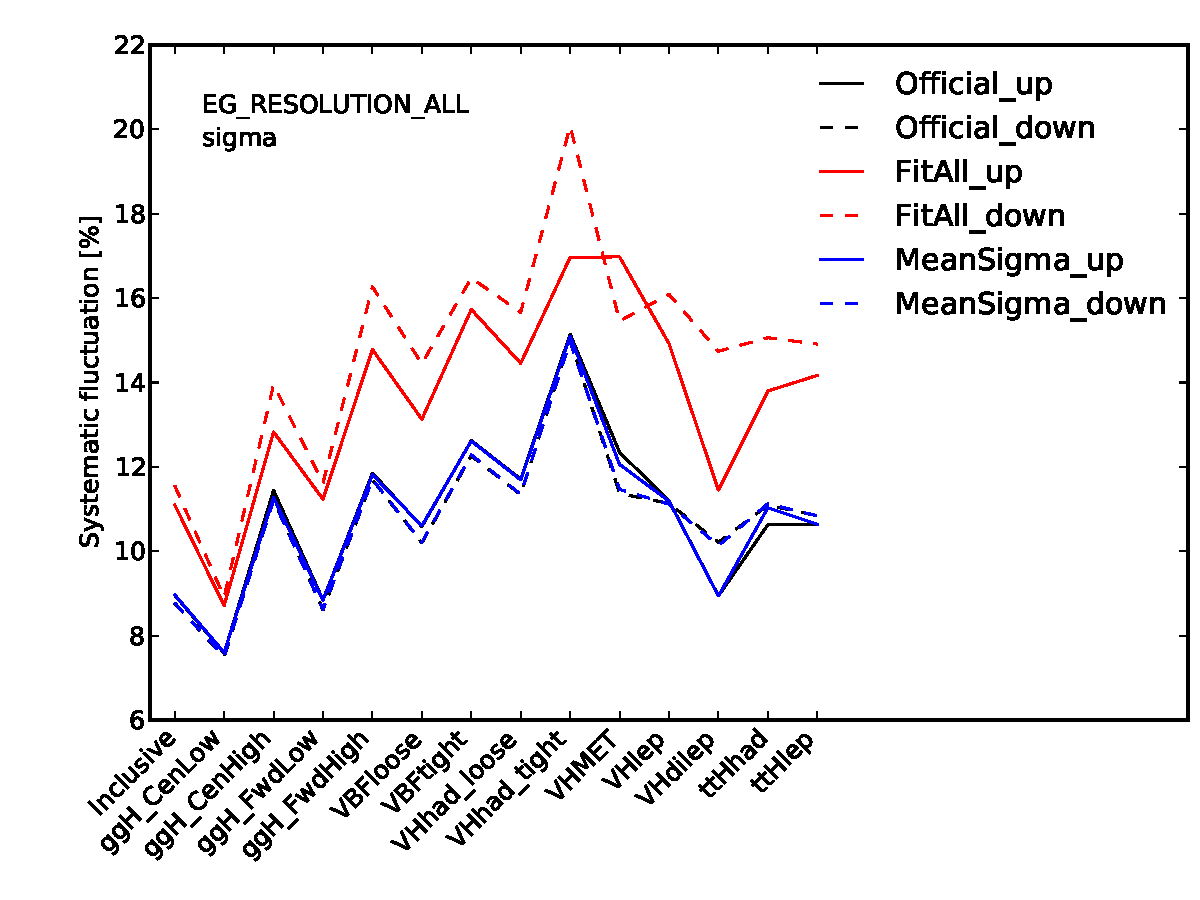
\includegraphics[width=\linewidth]{plots/Backup/h013_meanSigma_PhotonSyst_EG_RESOLUTION_ALL_sigma.pdf}\\
  \end{minipage}
  \hfill
  \begin{minipage}{0.59\linewidth}
    \begin{itemize}
    \item $\sigma$ is sensitive to the change of scale.
    \item Two understood explanations :
      \begin{itemize}
      \item $\mu /\sigma$ correlation when scaling energies.
      \item Resolution loss due to inhomogenous scaling.
        \end{itemize}
      \vfill
    \item Effect on resolution is small but I propose to \textcolor{red}{add a width effect linked to EG\_SCALE\_ALL nuisance parameter}.
      \begin{itemize}
      \item Add a second nuisance parameter to the width to limit overconstraints.
      \item Good hopes to reduce Zee resolution systematics (dominant in EG\_RESOLUTION\_ALL) within medium timescale.
      \end{itemize}
    \end{itemize}
  \end{minipage}
\end{frame}

%%=============================================================
\begin{frame}{Cross-check : template method}
\begin{minipage}{0.59\linewidth}
  The template method is used to measure $\alpha$ and $C$ simultaneously.
\begin{itemize}
\item Create distorded MC (templates) with test values of $\alpha$ and $C$.
\item \textcolor{blue}{\bf Compute $\chi^2$ between Z mass distribution of data and template}.
\item \textcolor{blue}{\bf Fit the minimum of the $\chi^2$ distribution} in the ($\alpha,C$) plane.
\item Fit performed in 2 steps of 1D fits : 
\begin{itemize}
\item fit $\chi^2=f(\alpha)$ at constant $C$ (lines) $\rightarrow (\alpha_{min}, \chi^2_{min})$ .
\item fit $\chi^2_{min}=f(C)\rightarrow (C, \Delta C)$
\item project $C$ in $\alpha_{min}=f(C)$, corresponding bin gives $(\alpha, \Delta\alpha)$.
\end{itemize}
\end{itemize}
  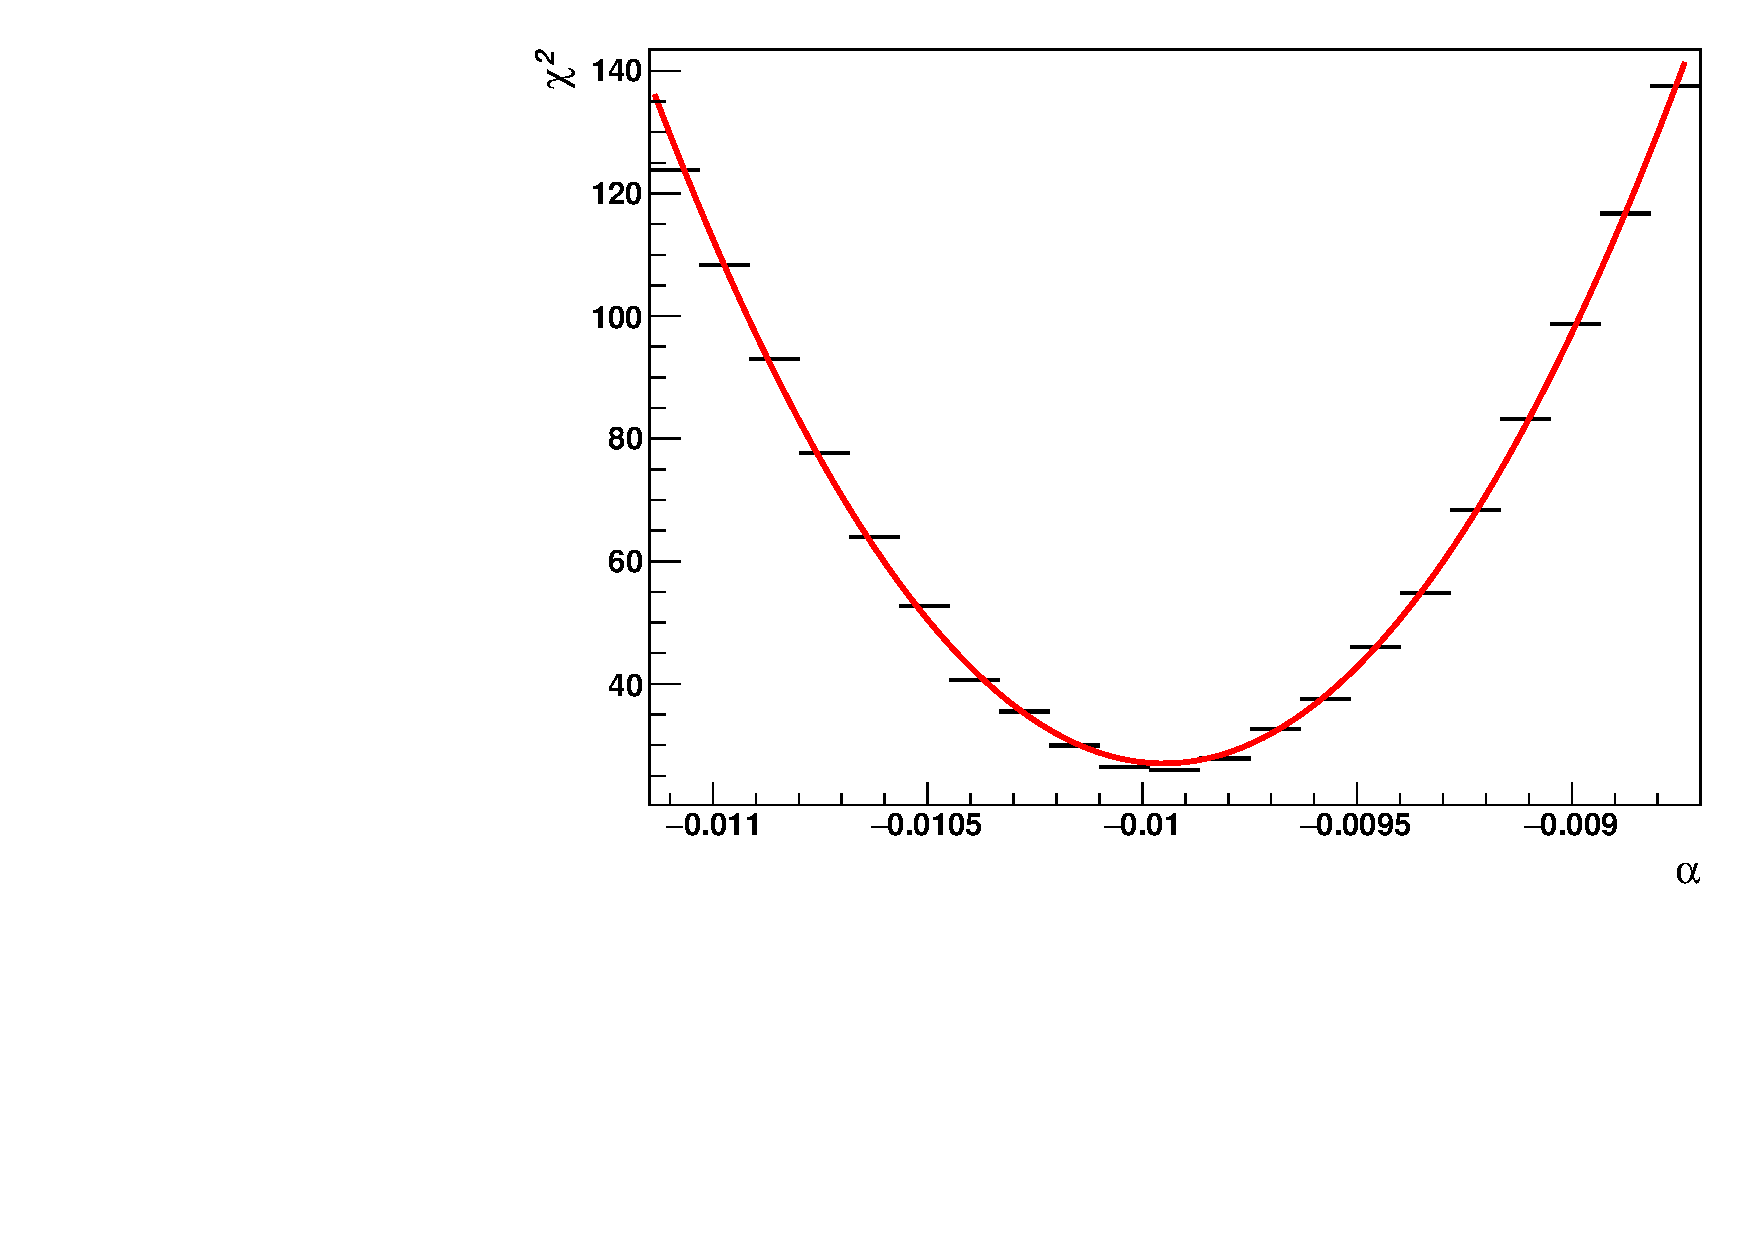
\includegraphics[width=0.325\linewidth]{plots/Backup/MC6_0_0_chi2FitNonConstVar_10.pdf}
  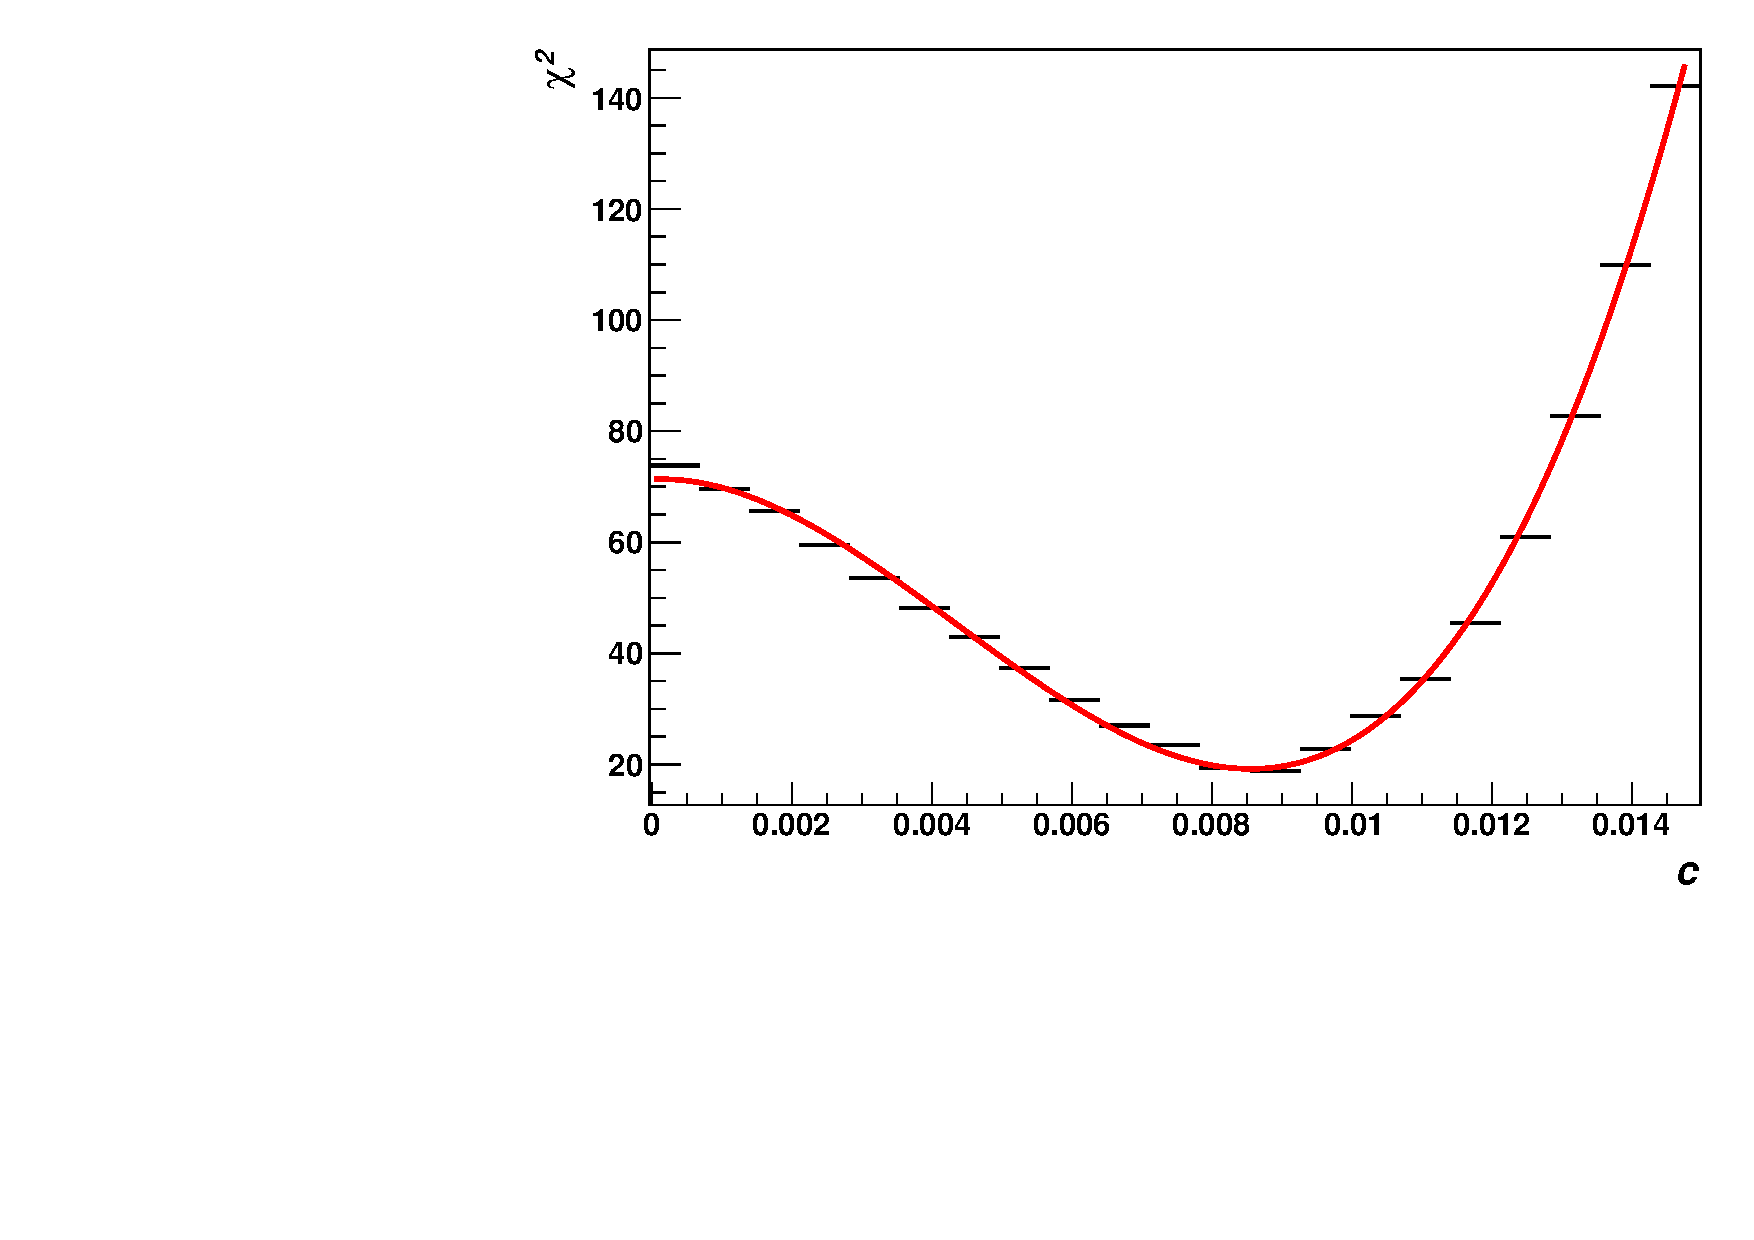
\includegraphics[width=0.325\linewidth]{plots/Backup/MC6_0_0_chi2FitConstVar.pdf}
  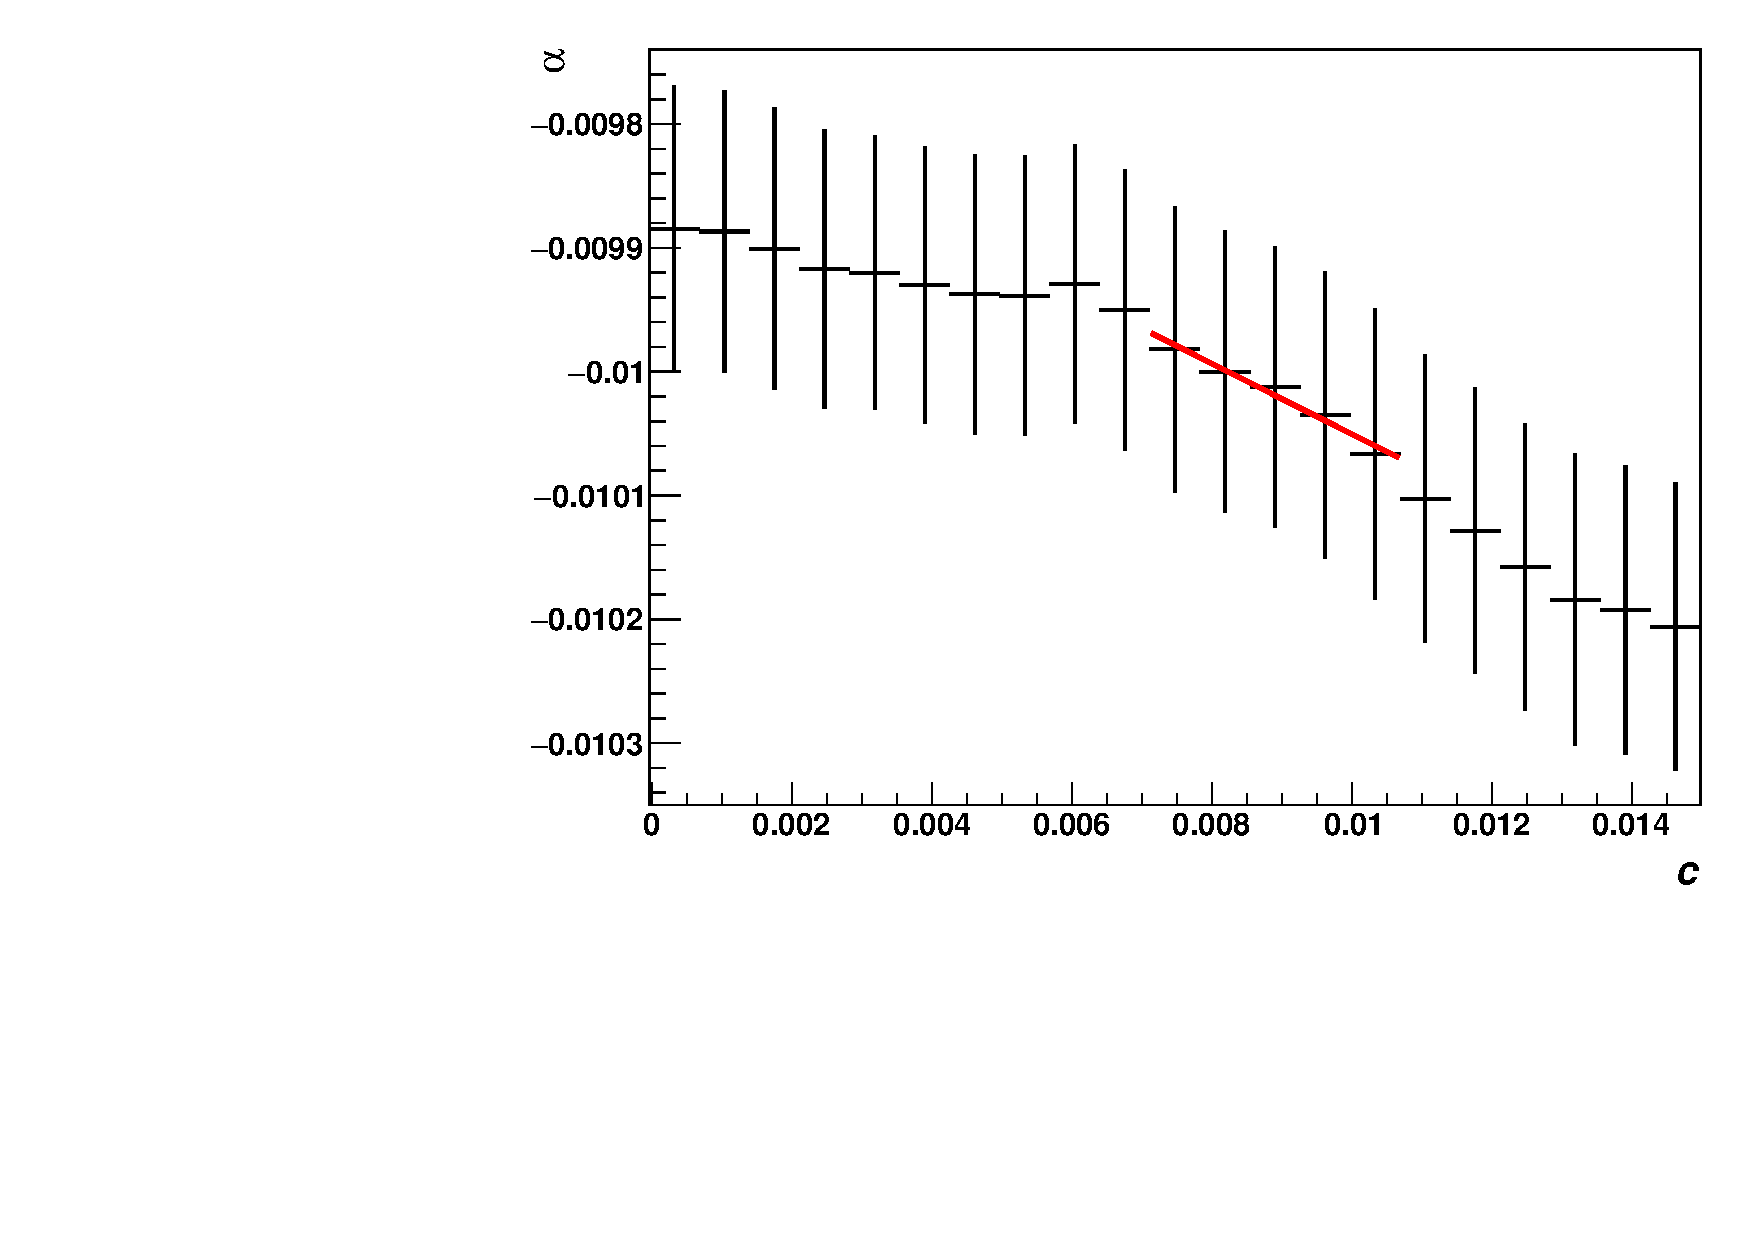
\includegraphics[width=0.325\linewidth]{plots/Backup/MC6_0_0_corAngle.pdf}
\end{minipage}
\hfill
\begin{minipage}{0.4\linewidth}
  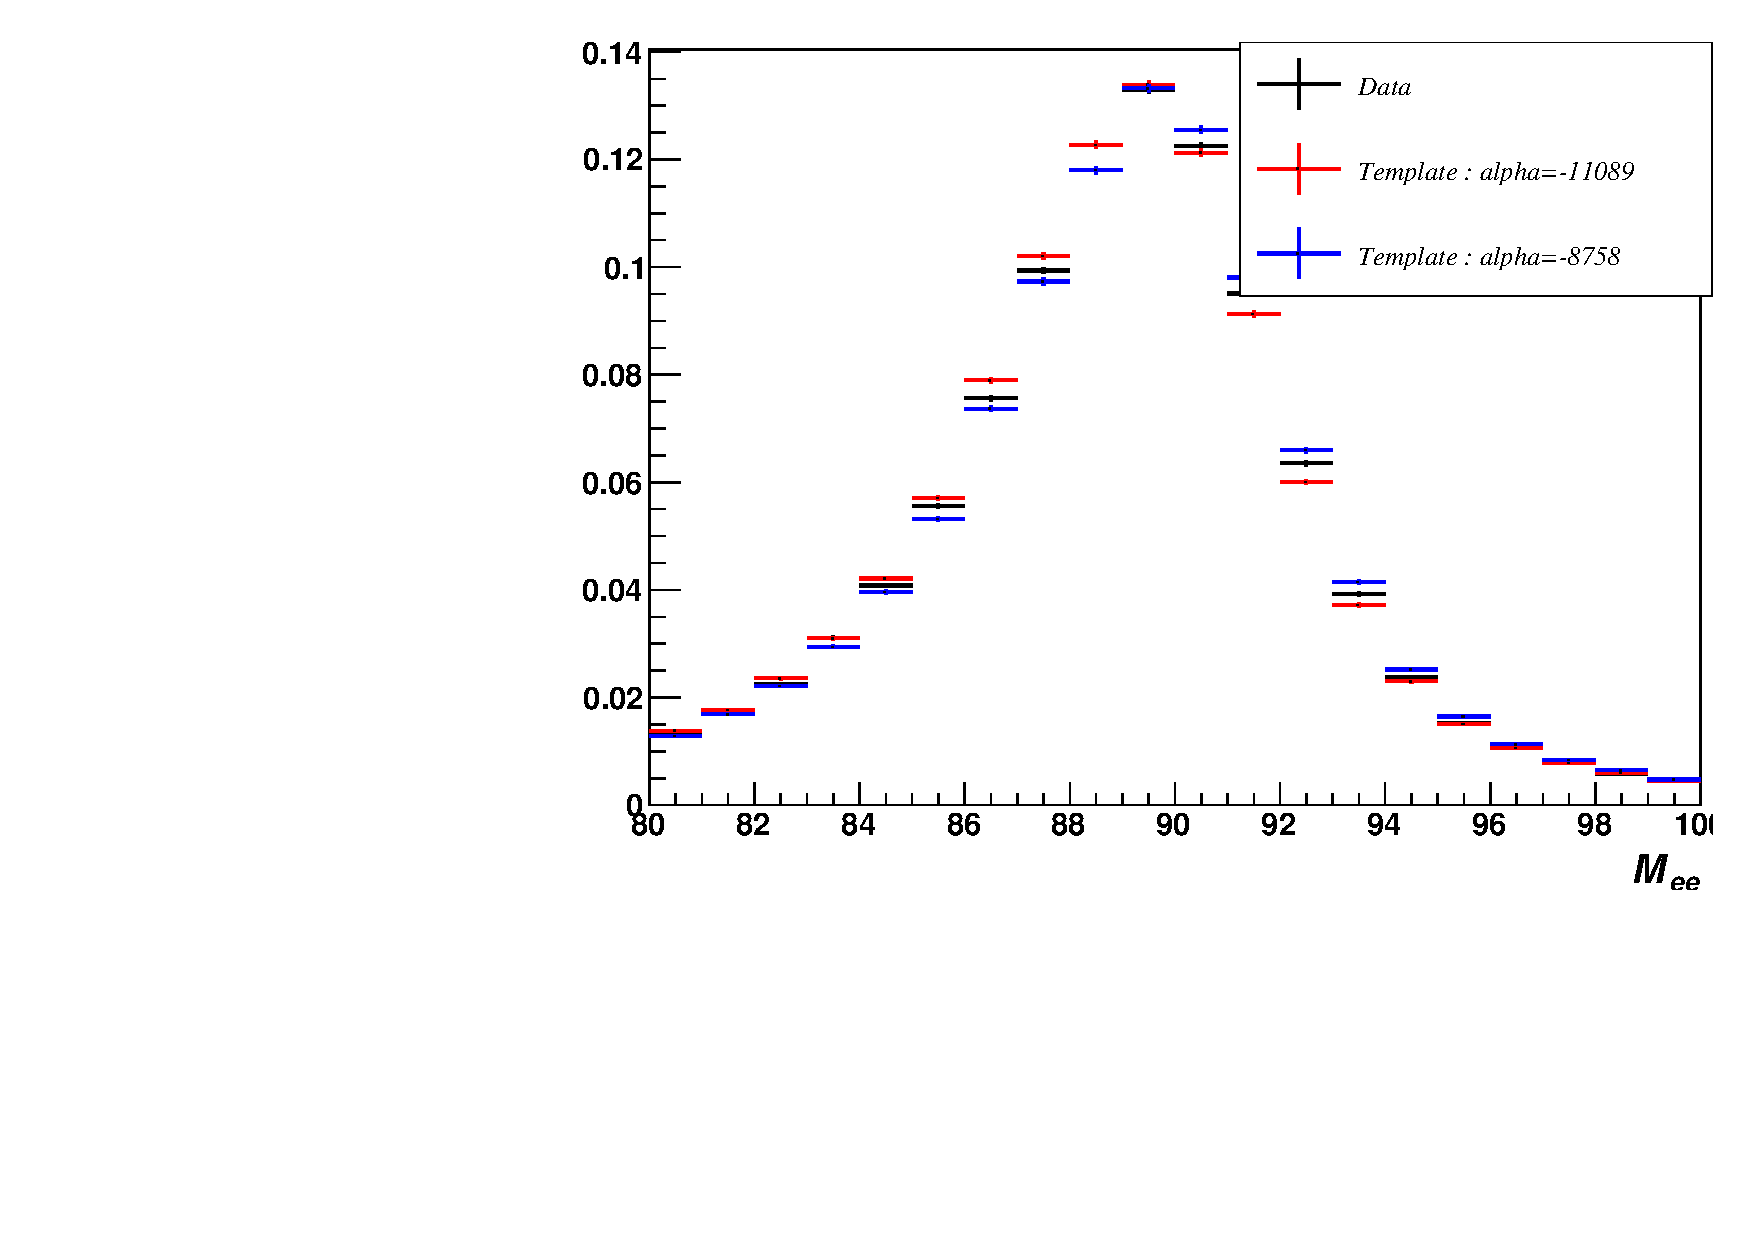
\includegraphics[width=\linewidth]{plots/Backup/MC6_0_0_CompareAlpha.pdf}\\
  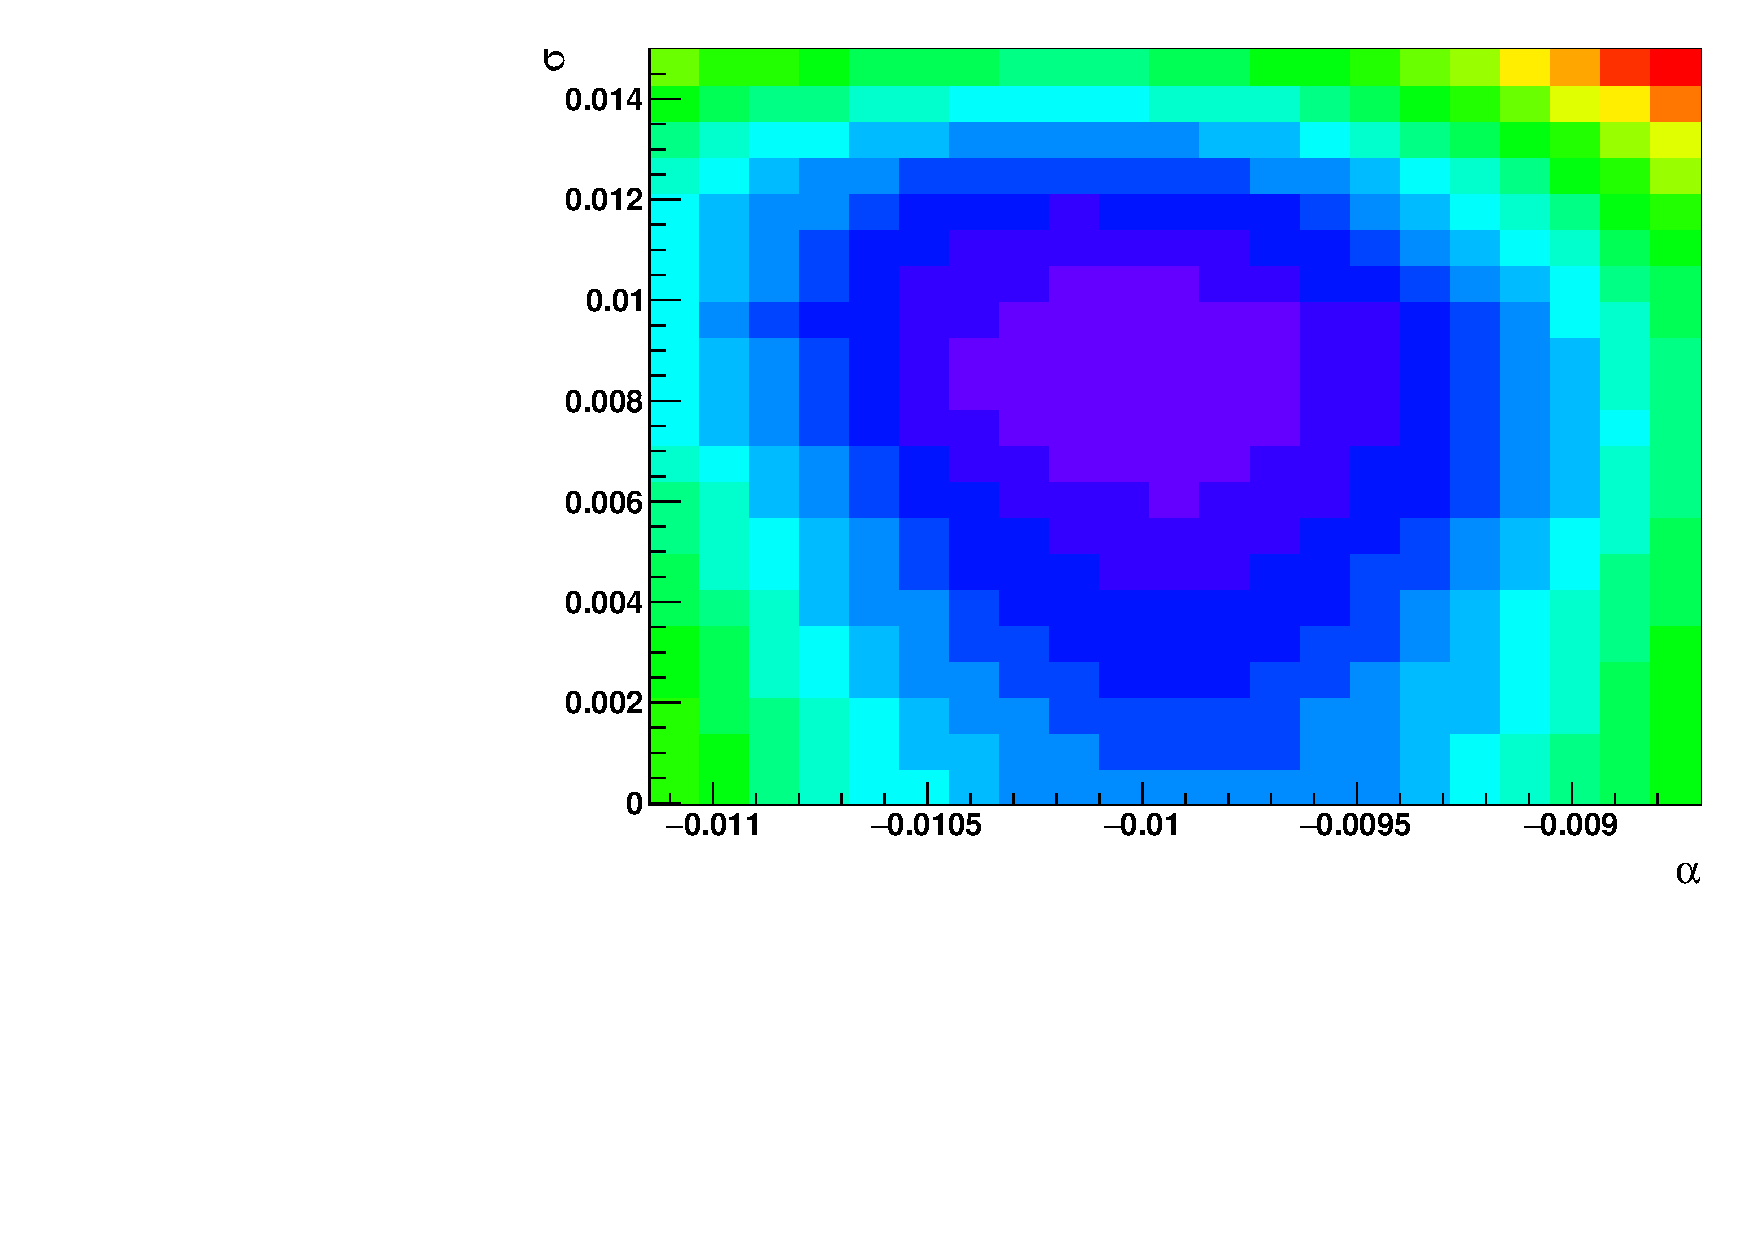
\includegraphics[width=\linewidth]{plots/Backup/MC6_0_0_chiMatrix.pdf}\\
\end{minipage}
\end{frame}

%==============================================================================
\begin{frame}{Scale factors interpretation}
  \begin{minipage}{0.49\linewidth}
    Assume the up fluctuation (red) as data and nominal distribution (black) as MC in the template method.
    One has
    $$m_H^{up}=m_H^{nom}(1+\alpha)$$
    Hence
    $$\delta_{m_H}=\alpha$$
    \end{minipage}
  \begin{minipage}{0.49\linewidth}
    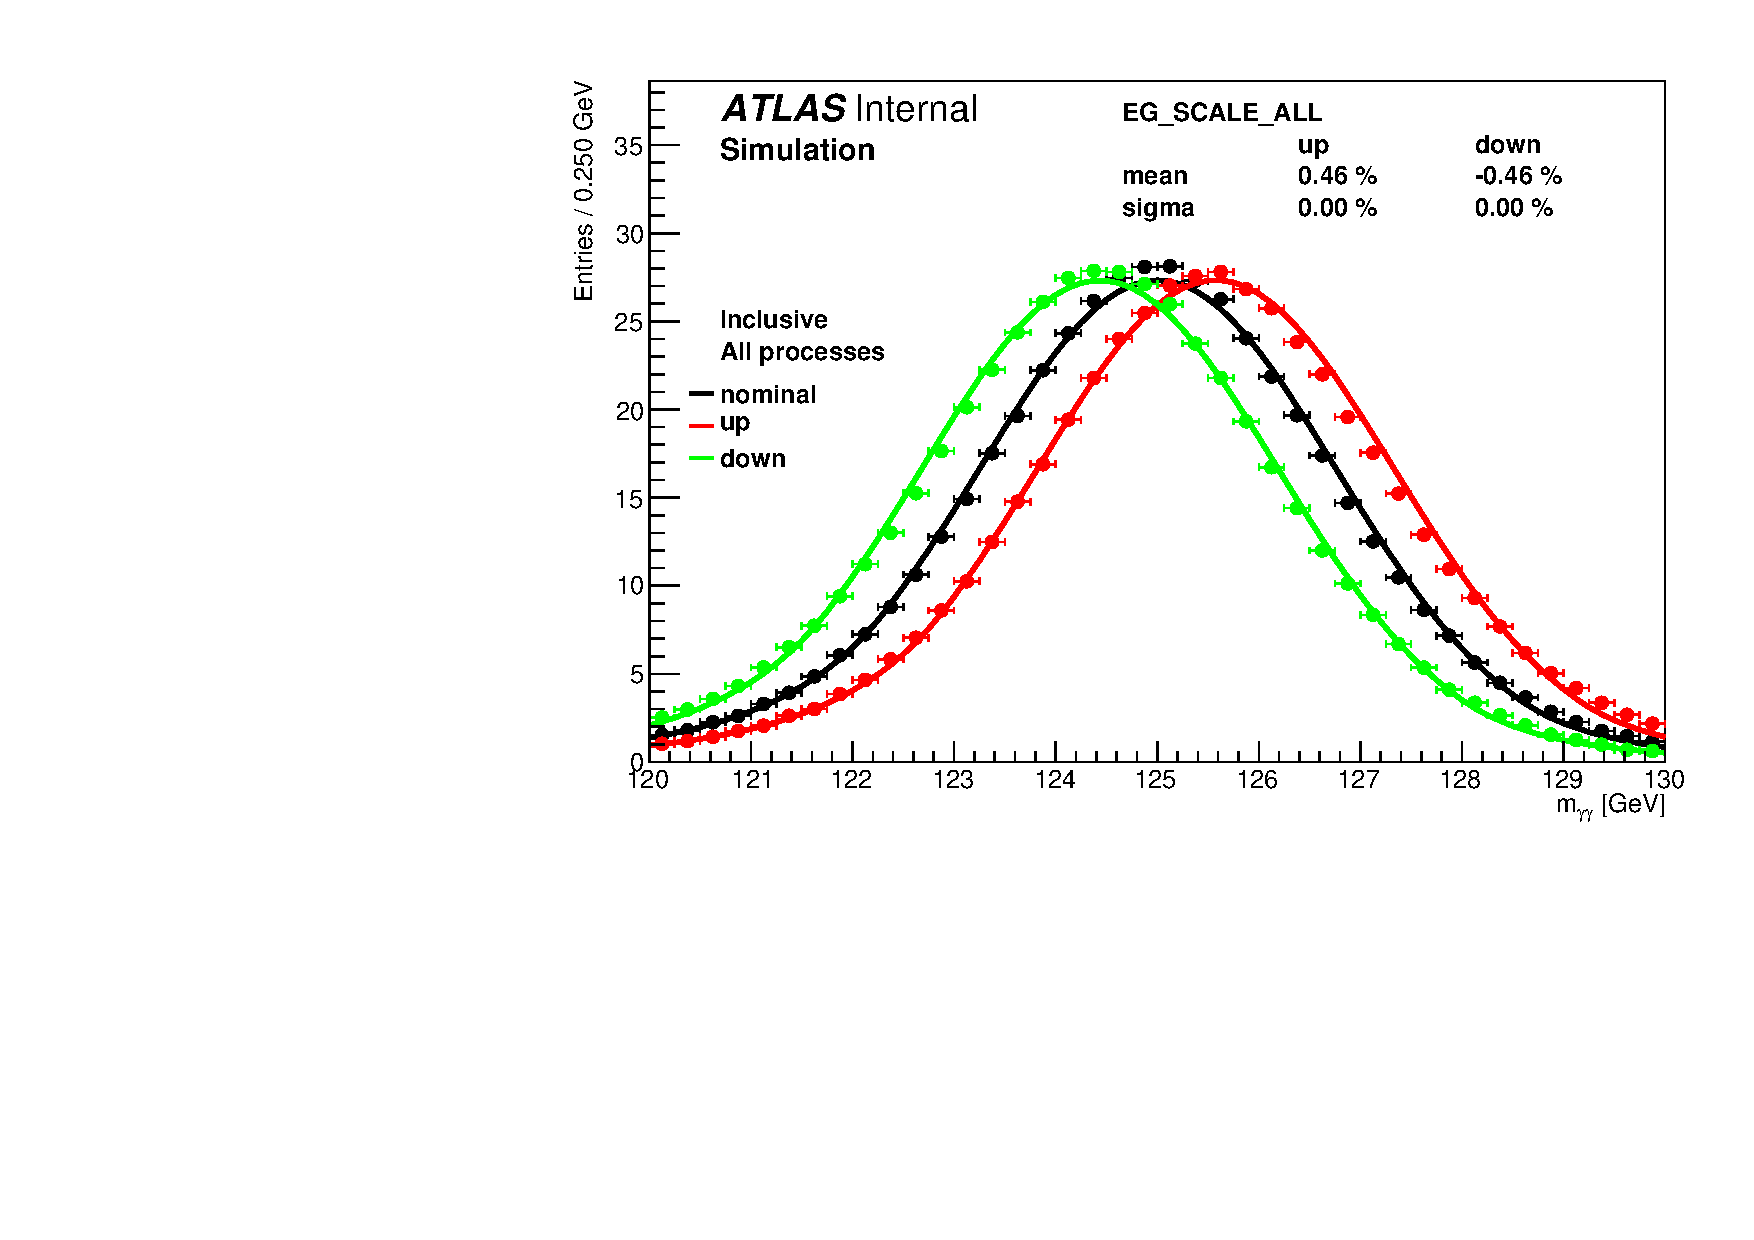
\includegraphics[width=\linewidth]{plots/Backup/h013_EG_SCALE_ALL_0.pdf}
  \end{minipage}
  Furthermore :
  $$\sigma_H^{up}=\sigma_H^{nom} \oplus cE$$
  Hence
  $$\delta_{\sigma_H} = \sqrt{1+\frac{c^2E^2}{\sigma_H^2}}-1$$
  One has to be carefull with resolution uncertainty as the template method is weak to measure small differences.
\end{frame}
